\documentclass[12pt,a4paper]{article}
\usepackage{amsmath}
\usepackage{graphicx}
\usepackage{geometry}
\usepackage{float}
\geometry{left=2cm,right=2cm,top=2.5cm,bottom=2.5cm}

\title{\textbf{Kinematic and Singularity Analysis Report \\ with Explicit Matrix Operations}}
\author{Automated Generation System}
\date{\today}

\begin{document}
\maketitle

\section{Mathematical Formulation \& Singularity Extraction}
The closed-loop spatial mechanism is driven by $q_1$, leaving $q_2 \dots q_7$ as 6 passive joints. To evaluate the structural singularity of the entire mechanism loop, we extract the passive Jacobian $J_p \in \mathbb{R}^{6 \times 6}$ corresponding to the remaining kinematics loop. 

By identifying the local minima of the 6th singular value ($\sigma_6$), the following critical singular configurations (dead centers) were numerically extracted:
\begin{itemize}
    \item Driven by $q_1 = 210.58^\circ$, the minimum singular value drops to $\sigma_6 = 0.001481$.
\end{itemize}

\section{Example Matrix Calculation at $q_1 = 0^\circ$}
The solved full joint configuration (in radians) is:
\begin{equation}
    \mathbf{q} = \begin{bmatrix} 0.0000 \\ 0.0276 \\ -0.0003 \\ -0.0552 \\ 0.0005 \\ -0.0276 \\ -0.0008 \end{bmatrix}
\end{equation}

The full $6 \times 7$ Jacobian matrix $J$:
\begin{equation}
    \resizebox{0.95\textwidth}{!}{$ J = \begin{bmatrix}
  0.000 & 0.000 & 0.000 & 2.499 & -0.069 & -2.501 & -0.000 \\
  0.000 & -1.000 & -0.000 & 2.999 & -0.000 & 1.997 & 0.000 \\
  -0.000 & 0.000 & -3.000 & 0.069 & -0.500 & 0.069 & -2.000 \\
  0.000 & 0.000 & 0.000 & 0.028 & 0.000 & 0.028 & -0.001 \\
  0.000 & 0.000 & -1.000 & -0.000 & -1.000 & 0.000 & 1.000 \\
  1.000 & 1.000 & 0.000 & -1.000 & 0.000 & 1.000 & 0.000
\end{bmatrix} $}
\end{equation}

The structural $6 \times 6$ passive Jacobian $J_p$ (excluding $J_1$):
\begin{equation}
    \resizebox{0.85\textwidth}{!}{$ J_p = \begin{bmatrix}
  0.000 & 0.000 & 2.499 & -0.069 & -2.501 & -0.000 \\
  -1.000 & -0.000 & 2.999 & -0.000 & 1.997 & 0.000 \\
  0.000 & -3.000 & 0.069 & -0.500 & 0.069 & -2.000 \\
  0.000 & 0.000 & 0.028 & 0.000 & 0.028 & -0.001 \\
  0.000 & -1.000 & -0.000 & -1.000 & 0.000 & 1.000 \\
  1.000 & 0.000 & -1.000 & 0.000 & 1.000 & 0.000
\end{bmatrix} $}
\end{equation}

Applying SVD on $J_p = U \Sigma V^T$ yields 6 singular values. The left singular vectors $U$:
\begin{equation}
    \resizebox{0.85\textwidth}{!}{$ U = \begin{bmatrix}
  0.665 & 0.106 & -0.635 & -0.002 & 0.379 & 0.002 \\
  0.671 & -0.031 & 0.738 & 0.007 & 0.068 & 0.011 \\
  0.064 & -0.983 & -0.097 & -0.142 & -0.002 & 0.000 \\
  0.005 & -0.001 & 0.009 & -0.000 & 0.012 & -1.000 \\
  0.010 & -0.140 & -0.023 & 0.990 & -0.011 & -0.000 \\
  -0.323 & -0.045 & 0.206 & 0.012 & 0.923 & 0.011
\end{bmatrix} $}
\end{equation}

The singular values matrix $\Sigma$ ($6 \times 6$):
\begin{equation}
    \resizebox{0.85\textwidth}{!}{$ \Sigma = \begin{bmatrix}
  4.178 & 0.000 & 0.000 & 0.000 & 0.000 & 0.000 \\
  0.000 & 3.672 & 0.000 & 0.000 & 0.000 & 0.000 \\
  0.000 & 0.000 & 3.351 & 0.000 & 0.000 & 0.000 \\
  0.000 & 0.000 & 0.000 & 1.669 & 0.000 & 0.000 \\
  0.000 & 0.000 & 0.000 & 0.000 & 0.892 & 0.000 \\
  0.000 & 0.000 & 0.000 & 0.000 & 0.000 & 0.000
\end{bmatrix} $}
\end{equation}

And $V^T$ ($6 \times 6$):
\begin{equation}
    \resizebox{0.85\textwidth}{!}{$ V^T = \begin{bmatrix}
  -0.238 & -0.048 & 0.957 & -0.021 & -0.153 & -0.028 \\
  -0.004 & 0.841 & 0.041 & 0.170 & -0.119 & 0.497 \\
  -0.159 & 0.094 & 0.123 & 0.035 & 0.973 & 0.051 \\
  0.003 & -0.338 & -0.004 & -0.550 & 0.013 & 0.763 \\
  0.958 & 0.018 & 0.258 & -0.016 & 0.123 & -0.008 \\
  -0.023 & 0.408 & -0.014 & -0.816 & 0.009 & -0.408
\end{bmatrix} $}
\end{equation}

\section{Analysis Results \& Curve Fitting}
\begin{figure}[H]
    \centering
    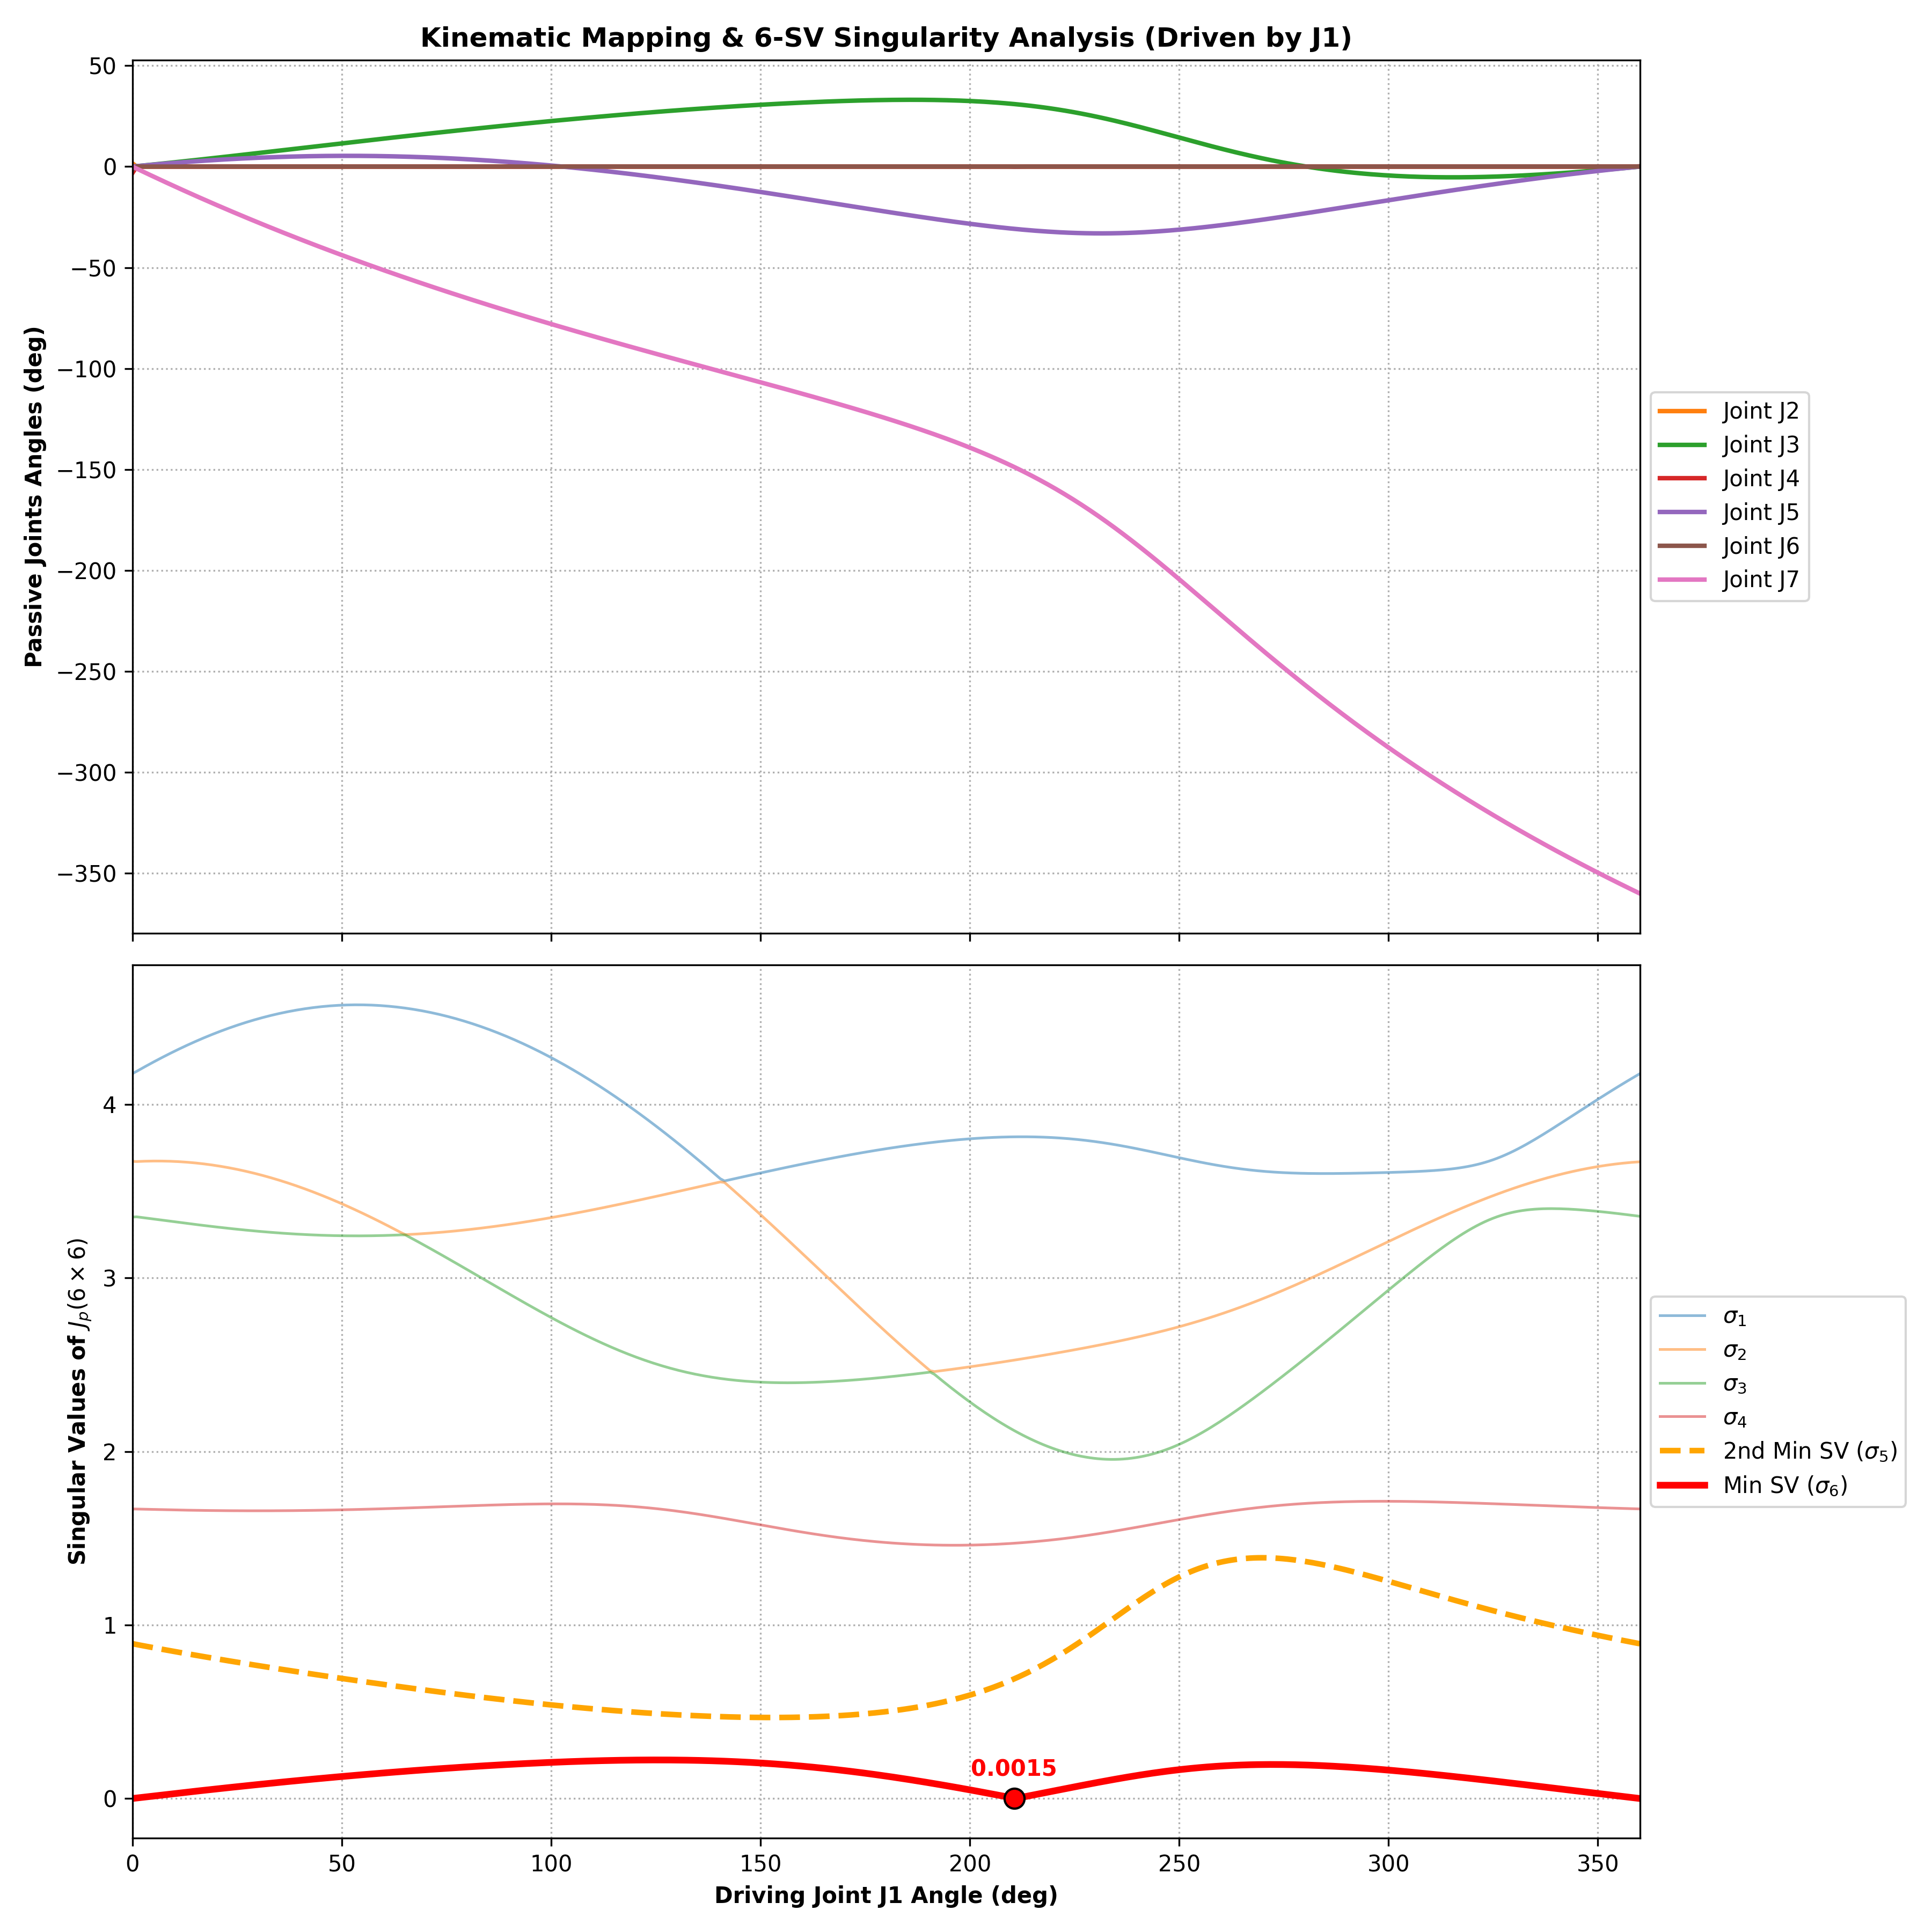
\includegraphics[width=0.9\textwidth]{j1_unconstrained_6sv_analysis.png}
    \caption{Kinematic mapping and full $6 \times 6$ singular value evolution. Critical dead centers are highlighted in red.}
\end{figure}

The 3rd-order Fourier series expressions for the passive joints are:
\begin{itemize}
\item \textbf{Joint J2:} \\ $Q_{J2}(x) = +0.004 +0.008\cos(x) -0.000\sin(x) +0.008\cos(2x) +0.001\sin(2x) +0.008\cos(3x) -0.001\sin(3x)$
\item \textbf{Joint J3:} \\ $Q_{J3}(x) = +14.740 -17.160\cos(x) +7.200\sin(x) +2.093\cos(2x) +3.424\sin(2x) +0.617\cos(3x) -0.949\sin(3x)$
\item \textbf{Joint J4:} \\ $Q_{J4}(x) = -0.009 -0.015\cos(x) +0.001\sin(x) -0.017\cos(2x) -0.001\sin(2x) -0.016\cos(3x) +0.001\sin(3x)$
\item \textbf{Joint J5:} \\ $Q_{J5}(x) = -11.728 +11.634\cos(x) +14.541\sin(x) +0.433\cos(2x) -1.922\sin(2x) -0.459\cos(3x) +0.224\sin(3x)$
\item \textbf{Joint J6:} \\ $Q_{J6}(x) = -0.004 -0.008\cos(x) +0.000\sin(x) -0.008\cos(2x) -0.001\sin(2x) -0.008\cos(3x) +0.001\sin(3x)$
\item \textbf{Joint J7:} \\ $Q_{J7}(x) = -153.532 -28.794\cos(x) +107.247\sin(x) +1.660\cos(2x) +62.635\sin(2x) +1.077\cos(3x) +37.015\sin(3x)$
\end{itemize}
\end{document}
